\section{Discord - Erub}

Discord est un logiciel propriétaire gratuit de VoIP et de messagerie instantanée. Il fonctionne sur les systèmes d’exploitation Windows, macOS, Linux, Android, iOS ainsi que sur les navigateurs web.

Pour développement de mon bot discord, je suis passée par l'API discord.\\

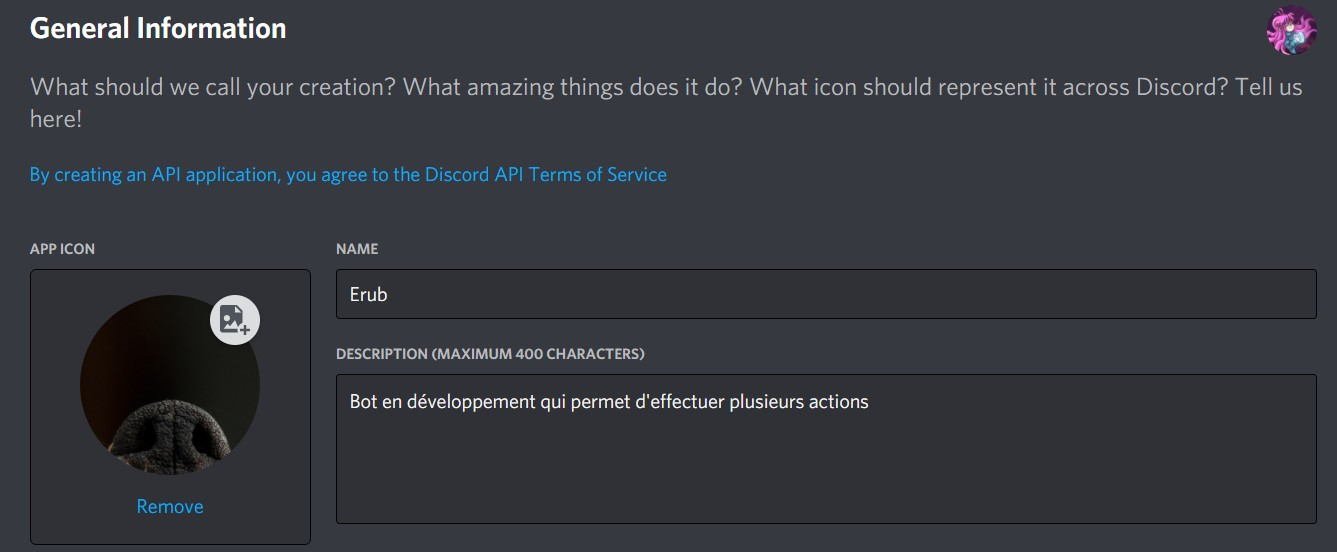
\includegraphics[width=16cm]{img/api.jpg}	

L'api permet d'avoir un token permettant de relier le bot que l'on développe à l'api pour permet au bot de rejoindre des serveurs. Le token est important, il ne faut pas rendre public.

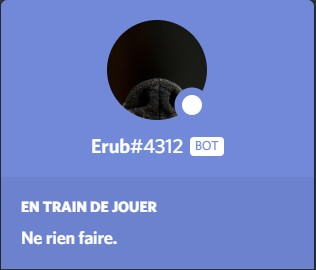
\includegraphics[width=5cm]{img/Erub.jpg}	

Structure de Erub: 
- commandes : Ce dossier contient toutes les focntionnalitées du bot triées dans d'autres dossiers.

- config.js : Contient les paramètres a initiliser si vous voulez tester le bot sur votre serveur.

- node\_modules : contient tous les packages node js dont nous avons besoin

- package.json : contient les dépendences et leur version ainsi que des scripts

- main.js : Point d'entrée de l'application.

J'ai appris à mettre des statuts personnalisées sur mon bot. 
Cela peut permettre à des utilisateurs ne connaissant pas le bot d'avoir des informations, par exemple j'affiche la commade "?help"

Erub peut également afficher un message de bienvenue aux utilisateurs pour cela il suffit de mettre l'id du channel dans le config.js

Il peut également afficher les sondages dans un channel dédier ou alors la ou vous taper la commande si vous initialisez à num le paramètre "CHANNEL\_POLL" dans le fichier config.json.
